<<<<<<< HEAD
\section{Auswertung}
\label{sec:Auswertung}
\subsection{Wheatstonesche Brücke}
In den Tabellen \ref{tab:11} und \ref{tab:14}
sind die eingestellten Werte der
Wheatstoneschen Brücke für unterschiedliche $R_2$ aufgelistet.
Dadurch kann der unbekannte Widerstand $R_\mathrm{x}$ mit der
Formel \eqref{eqn:} berechent werden.
\begin{table}
 \centering
 \caption{Bestimmung des Wiederstandes des Wiederstand 11.}
 \label{tab:11}
  \begin{tabular}{c c c c c}
\toprule
$R_3/\si{\ohm} $& $R_4/\si{\ohm}$ & $\frac{R_3}{R_4} $ & $ R_2/\si{\ohm} $ & $R_\mathrm{x}/\si{\ohm}  $ \\
\midrule
604,0 & 396,0 & 1,525\pm0,008 & 332\pm10 & 506,4\pm15,4\\
427,0 & 573,0 & 0,745\pm0,004 & 664\pm20 & 494,8\pm15,0\\
330,0 & 670,0 & 0,493\pm0,002 & 1000\pm30 & 492,5\pm15,0\\
\bottomrule
\end{tabular}
\end{table}

\begin{table}
 \centering
 \caption{Bestimmung des Wiederstandes des Wiederstand 14.}
 \label{tab:14}
  \begin{tabular}{c c c c c}
\toprule
$R_3/\si{\ohm} $& $R_4/\si{\ohm}$ & $\frac{R_3}{R_4} $ & $ R_2/\si{\ohm} $ & $R_\mathrm{x}/\si{\ohm}  $ \\
\midrule
739 & 261 & 2,83\pm0,01 &   332\pm10 &  940\pm29\\
585 & 415 & 1,410\pm0,007 & 664\pm20 &  936\pm28\\
482 & 512 & 0,941\pm0,005 & 1000\pm30 & 941\pm29\\
\bottomrule
\end{tabular}
\end{table}

Nun werden die Werte für die unterschiedlichen $R_\mathrm{x}$ gemittelt und
es ergeben sich die gemessenen Wiederstände:
\begin{align*}
R_11=   (497,9\pm8,7)\,\si{\ohm}
R_14=(939)\,\si{\ohm}
\end{align*}

\subsection{Kapazitätsmessbrücke}
Die Tabellen \ref{tab:1} und \ref{tab:2} enthalten
die Messwerte zur Bestimmung der Kapazität zweier
Kondensatoren.
Da es sich bei diese um hochwertigen Kondensatornen
handelt, kann auf den $R_2$ Widerstand
verzichtet werden.
Zur Fehlerbestimmung wird der Kondensator $C_2$ variiert
und mit der Formel \eqref{eqn:  } lässt sich
aus den Messwerten die Kapaitäten $C_\mathrm{x}$ für die einzelnen
Kondensatoren bestimmen.
\begin{table}
 \centering
 \caption{Bestimmung der Kapazität des Kondensators 1.}
 \label{tab:3}
  \begin{tabular}{c c c c c}
\toprule
$R_3/\si{\ohm} $& $R_4/\si{\ohm}$ & $\frac{R_3}{R_4} $ & $ C_2/\si{\nano\farad} $ & $C_\mathrm{x}/\si{\nano\farad}  $ \\
\midrule
406,0 & 594,0 & 0,684 \pm 0,003 & 459\pm1 & 671,5\pm3,6 \\
537,0 & 263,0 & 2,04\pm0,01 & 750\pm2 & 367,3\pm2,0 \\
610,0 & 390,0 & 1,564\pm0,008 & 994\pm2 & 635,5\pm3,4 \\
\bottomrule
\end{tabular}
\end{table}

\begin{table}
 \centering
 \caption{Bestimmung der Kapazität des Kondensators 3.}
 \label{tab:3}
  \begin{tabular}{c c c c c}
\toprule
$R_3/\si{\ohm} $& $R_4/\si{\ohm}$ & $\frac{R_3}{R_4} $ & $ C_2/\si{\nano\farad} $ & $C_\mathrm{x}/\si{\nano\farad}  $ \\
\midrule
525 & 475 & 1,105\pm 0,006 & 450\pm1  & 407,1\pm 2,2\\
647 & 353 & 1,833\pm 0,009 & 750\pm2  & 409,2\pm 2,2\\
712 & 282 & 2,526\pm 0,01  & 994\pm2  & 393,7\pm 2,1\\
\bottomrule
\end{tabular}
\end{table}

\FloatBarrier
Werden die bestimmten Kapazitäten gemittelt
ergibt sich für
\begin{align*}
  C_1&=(558,1\pm1,8)\,\si{\nano\farad}
\intertext{und}
  C_3&=(403,3\pm1,3)\,\si{\nano\farad}.
\end{align*}

In Tabelle \ref{tab:8} sind die Messwerte
für eine RC-Kombination
aufgetragen. Da ebenfalls der Widerstand $R_\mathrm{x}$
bestimmt wird, wird ein Stellglied $R_2$ verwendet. Wie
bei den anderen Messungen auch wird wieder $C_2$ variiert.
\begin{table}
 \centering
 \caption{Bestimmung des Wiederstandes und der Kapazität der RC-Kombination 8.}
 \label{tab:8}
  \begin{tabular}{c c c c c c c}
\toprule
$R_3/\si{\ohm}$ & $R_4/\si{\ohm}$ & $\frac{R_3}{R_4}$ & $R_2/\si{\ohm}$ & $L_2/\si{\nano\farad} $ & $ R_\mathrm{x}/\si{\ohm} $ & $C_\mathrm{x}/\si{\nano\farad} $\\
\midrule
612 & 388 & 1,58\pm0,01 & 377\pm11 & 450\pm1 & 594,6\pm18,1 & 285,3\pm1,5\\
725 & 275 & 2,64\pm0,01 & 229\pm7  & 750\pm2 & 603,7\pm18,4 & 284,5\pm1,5\\
781 & 219 & 3,57\pm0,02 & 170\pm5  & 994\pm2 & 606,3\pm18,4 & 278,7\pm1,5\\
\bottomrule
\end{tabular}
\end{table}

Für die gemittelte Kapazität ergibt sich
\begin{align*}
 C_8=(282,8\pm0,9)\,\si{\nano\farad}
\intertext{und der gemittelte Widerstand beträgt:}
 R_8=(601,5\pm10,6)\,\si{\ohm}
\end{align*}
\subsection{Induktivitätsmessbrücke}
Nun wird die die Induktiviät und Widerstand einer
RL-Kombination mit der Induktivitätsmessbrücke bestimmt.
Die Tabelle \ref{tab:17} enthält die Einstellung
der Brücke und sowohl die aus Formel \eqref{eqn:}
berechente Induktivität
$L_x$ als auch den aus Formel
\eqref{eqn:} berechneten Widerstand $R_x$.
Zur Fehlerbestimmung wird $L_2$ varriert.
\begin{table}
 \centering
 \caption{Bestimmung des Wiederstandes und der Induktivität der RL-Kombination 17.}
 \label{tab:17}
  \begin{tabular}{c c c c c c c}
\toprule
$R_3/\si{\ohm}$ & $R_4/\si{\ohm}$ & $\frac{R_3}{R_4}$ & $R_2/\si{\ohm}$ & $L_2/\si{\milli\henry} $ & $ R_x/\si{\ohm} $& $L_x/\si{\milli\henry} $\\
\midrule
753,0 & 247,0 & 3,06\pm0,02   & 33,0\pm1,0 & 14,60\pm0,03 & 100,6\pm3,1 & 44,5\pm0,2\\
689,0 & 311,0 & 2,22\pm0,01   & 40,0\pm1,2 & 20,10\pm0,04 & 88,6\pm2,7  & 44,5\pm0,2\\
617,0 & 383,0 & 1,611\pm0,008 & 61,0\pm1,8 & 27,50\pm0,06 & 98,3\pm3,0  & 44,3\pm0,2\\
\bottomrule
\end{tabular}
\end{table}

Für die gemittelte Induktivität
ergibt sich:
\begin{align*}
  L_{17}&=(44,45\pm0,14)\,\si{\milli\henry}
\intertext{Der gemittelte Widerstand beträgt:}
R_{17}&=(95,8\pm1,7)\,\si{\ohm}
\end{align*}
\subsection{Maxwell-Brücke}
Die Induktivität und der Widerstand
der gleiche RL-Kombination wird
diesmal mit der Maxwwell-Brücke bestimmt. Die
Einstellung der Brücke sind in der Tabelle \ref{tab:17m}
aufgelistet mit den aus den Formeln
\eqref{eqn:} und \eqref{eqn:} berechenten Werte für
die Induktion und den Widerstand.
\begin{table}
 \centering
 \caption{Bestimmung des Wiederstandes und der Induktivität der RL-Kombination 17 mit Hilfe der Maxwell-Brücke.}
 \label{tab:17m}
  \begin{tabular}{c c c c c c c}
\toprule
$R_3/\si{\ohm}$ & $R_4/\si{\ohm}$ & $R_2/\si{\ohm}$ & $C_4\si{\nano\farad}$ & $ R_x/\si{\ohm} $& $L_x/\si{\milli\henry} $\\
\midrule
96\pm3  & 1009\pm30 & 1000\pm30 & 450\pm0,9 & 95\pm5 & 43,5888\pm2\\
45\pm1  & 1010\pm30 & 664\pm20  & 450\pm0,9 & 30\pm2 & 20,4525\pm1\\
290\pm9 & 1013\pm30 & 332\pm10  & 450\pm0,9 & 95\pm5 & 132,1965\pm6\\
\bottomrule
\end{tabular}
\end{table}

Der gemittelte Wert für die Induktion der
RL-Kombination beträgt:
\begin{align*}
  L_{17}=(65,4\pm2,0)\,\si{\milli\henry}.
\intertext{Für den gemittelten Widerstand ergibt sich ein Wert von:}
  R_{17}=(73,3\pm1,7)\,\si{\ohm}
\end{align*}

\subsection{TT-Brücke}
Die TT-Brücke enthält als Widerstände $R$  Widerstände
der Größe
\begin{align*}
R_\mathrm{TT}&=(1000\pm30)\,\si{\ohm}
\intertext{und die Kondensatoren $C$ besitzen die Kapazität}
C_\mathrm{TT}&=(403,3\pm1,3)\,\si{\nano\farad}.
\intertext{Als Eingangsspannung $U_\mathrm{S}$ wird eine Spannung von}
U_\mathrm{S}&=1,65\,\si{\volt}
\end{align*}
gemessen. In der Tabelle \ref{tab:TT}
sind die Ausgangsspannungen $U_{Br}$ für unterschiedlichen
Frequenzen $\nu$ aufgelistet.
\begin{table}
  \centering
  \caption{Messwerte für die Ausgangsspannung $U_{Br}$ bei unterschiedlichen Frequenzen $\nu$.}
  \label{tab:TT}
  \begin{tabular}{c c}
    \toprule
  $\nu/\si{\hertz}$ & $U_\mathrm{Br}/\si{\volt} $\\
    \midrule
    20       &   1,65\\
    50       &   1,5\\
    80       &   1,25\\
    100      &   1,1\\
    140      &   0,85\\
    170      &   0,7\\
    200      &   0,54\\
    220      &   0,46\\
    250      &   0,39\\
    280      &   0,26\\
    310      &   0,17\\
    340      &   0,1\\
    360      &   0,047\\
    380      &   0,005\\
    384      &   0,009\\
    400      &   0,041\\
    450      &  0,14\\
    500      &   0,23\\
    800      &   0,61\\
    1000     &  0,79\\
    2000     &   1,2\\
    5000     &   1,45\\
    10000    &   1,5\\
    18000    &   1,5\\
    28000    &   1,5\\
    30000    &  1,5\\
    \bottomrule
  \end{tabular}
\end{table}
Die Werte aus der Tabelle \ref{tab:TT}
werden nun in der Abbildung \ref{abb:TT}
in der Form $U_\mathrm{Br}/U_\mathrm{S}$
in Abhängigkeit von $\Omega$ aufgetragen.
Wobei
\begin{align*}
\Omega=\frac{\nu}{\nu_0}
\intertext{ist und das gemessene $\nu$ beträgt}
\nu_0=380\,\si{\hertz}.
\end{align*}
Die Abbildung \ref{abb:TT} enthält ebenfalls
eine Theoriekurve, die mit Hilfe der Formel
\eqref{eqn:TT} berechnet wird.
Aus den Werten für die Kapazität  $C_\mathrm{TT}$ und
den Widerstand $R_\mathrm{TT}$, ergibt sich ein Kreisfrequenz von
\begin{align*}
  \omega_0&=\frac{1}{RC}=(2480\pm70)\,\si{\hertz}.
\intertext{Daraus kann die theoretische Frequenz $v_\mathrm{0-Theorie}$ berechnet werden.}
\nu_\mathrm{0-Theorie}&=2\pi\cdot\omega_0=(394,6\pm11,9)\,\si{\hertz}
\end{align*}
Folglich beträgt $\Omega$ für die Theoriekurve:
\begin{align*}
  \Omega=\frac{\nu}{\nu_\mathrm{0-Theorie}}
\end{align*}
\begin{figure}
  \centering
  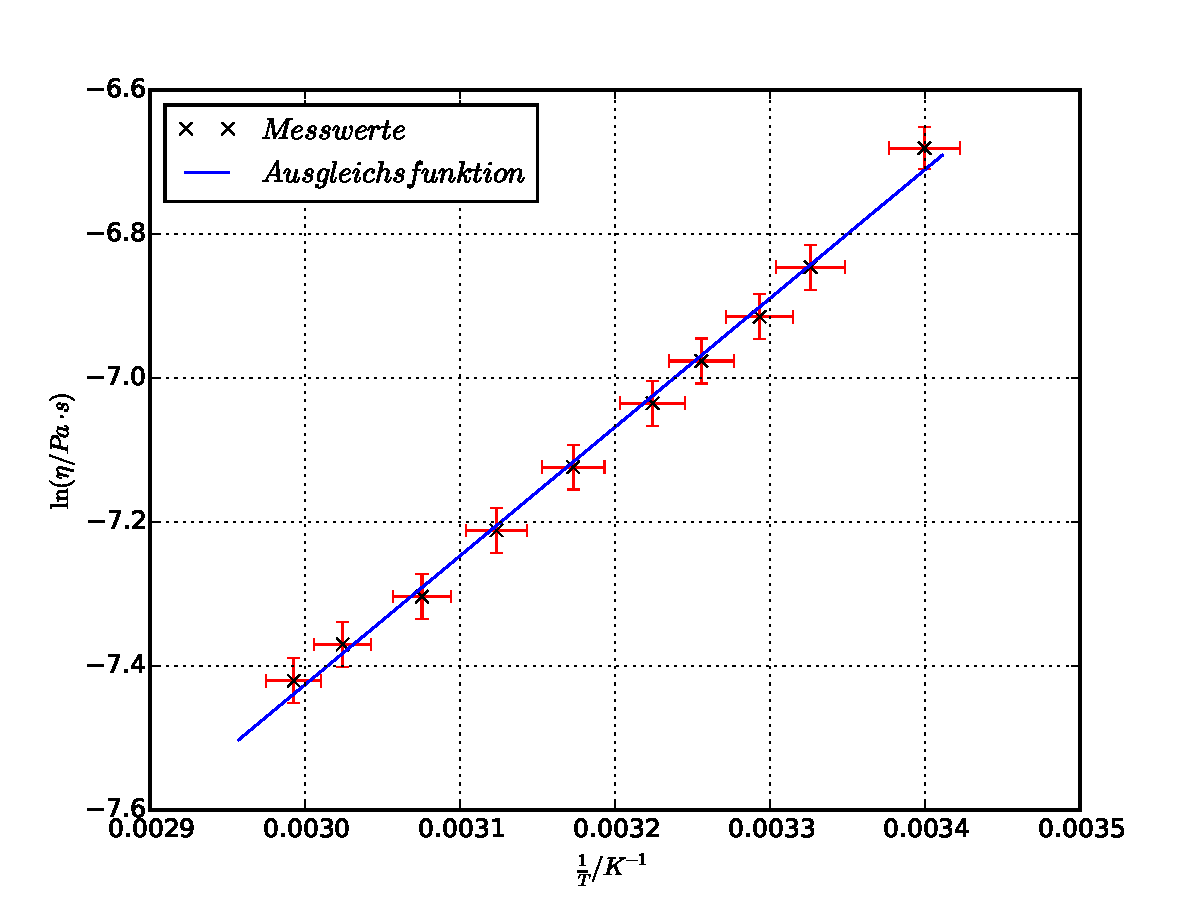
\includegraphics[width=0.7\textwidth]{plot.pdf}
  \caption{Messwerte und Theoriekurve für $U_\mathrm{Br}/U_\mathrm{S}$ in Abhängikeit von der Frequenz $\nu$ bei der TT-Brücke.}
  \label{abb:TT}
\end{figure}
\subsection{Bestimmung des Klirrfaktor}
Für die Bestimmung des Klirrfaktors wird
die Formel \eqref{eqn:klirr}
verwendet. Dabei wird zur Vereinfachung
angenommen, dass die Summe der Oberwellen
nur aus der Zweite Oberwelle besteht.
Somit gilt für den Klirrfaktor:
\begin{align}
  k=\frac{U_2}{U_1}\label{eqn:kcool}
\end{align}
Die Spannung $U_1$ ist das zuvor gemessene $U_\mathrm{S}$
und $U_2$ wird aus der Formel
\begin{align*}
  U_2=\frac{U_{Br_{min}}}{f(2)}
\end{align*}
berechnet. Hierbei ist $U_{Br_{min}}$ das
gemessene Minimum der
Brückenspannung:
\begin{align*}
U_{Br_{min}}=0,005\,\si{\volt}\\
\intertext{Die Funktion $f(2)$ ist die Formel \eqref{eqn:TT} mit einem $\Omega$ von 2. Somit folgt für $U_2$:}
U_2=\frac{0,005}{\sqrt{\frac{(2^2-1)^2}{(1-2^2)^2+16\cdot2^2}}}=0,014\,\si{\volt}
\intertext{und durch einsetzen in die Formel \eqref{eqn:kcool} ergibt sich ein Klirrfaktor von:}
k=0,0086
\end{align*}
||||||| merged common ancestors
=======
\section{Auswertung}
\label{sec:Auswertung}
>>>>>>> theorie und durchführung
